%----------------------------------------------------------------------------------------
%	PACKAGES AND THEMES
%----------------------------------------------------------------------------------------
\documentclass[aspectratio=169,xcolor=dvipsnames, t]{beamer}
\usepackage{fontspec} % Allows using custom font. MUST be before loading the theme!
\usetheme{SimplePlusAIC}
\usepackage{hyperref}
\usepackage{graphicx} % Allows including images
\usepackage{booktabs} % Allows the use of \toprule, \midrule and  \bottomrule in tables
\usepackage{svg} %allows using svg figures
\usepackage{tikz}
\usepackage{makecell}
\usepackage{wrapfig}

% ADD YOUR PACKAGES BELOW

%----------------------------------------------------------------------------------------
%	TITLE PAGE CONFIGURATION
%----------------------------------------------------------------------------------------

\title[Construction of the code]{Algebraic Geometric Codes} % The short title appears at the bottom of every slide, the full title is only on the title page
\subtitle{Construction of the code}

\author{Shree Ganesh S J \and Soham Chatterjee}
\institute[CMI]{Chennai Mathematical Institute}
% Your institution as it will appear on the bottom of every slide, maybe shorthand to save space


\date{\today} % Date, can be changed to a custom date
%----------------------------------------------------------------------------------------
%	PRESENTATION SLIDES
%----------------------------------------------------------------------------------------

\begin{document}

\maketitlepage

\begin{frame}[t]{Overview}
    % Throughout your presentation, if you choose to use \section{} and \subsection{} commands, these will automatically be printed on this slide as an overview of your presentation
    \tableofcontents
\end{frame}

%------------------------------------------------
% Section divider frame
\makesection{Basic blocks}

%------------------------------------------------
% Bullets
\begin{frame}{Bullet Points}
    \begin{itemize}
        \item Lorem ipsum dolor sit amet, consectetur adipiscing elit
        \item Aliquam blandit faucibus nisi, sit amet dapibus enim tempus eu
        \item Nulla commodo, erat quis gravida posuere, elit lacus lobortis est, quis porttitor odio mauris at libero
        \item Nam cursus est eget velit posuere pellentesque
        \item Vestibulum faucibus velit a augue condimentum quis convallis nulla gravida
        \item Nam cursus est eget velit posuere pellentesque
        \item Vestibulum faucibus velit a augue condimentum quis convallis nulla gravida
    \end{itemize}
\end{frame}

%------------------------------------------------
% Lists
\begin{frame}{Numbered List}
    \begin{enumerate}
        \item Lorem ipsum dolor sit amet, consectetur adipiscing elit
        \item Aliquam blandit faucibus nisi, sit amet dapibus enim tempus eu
        \item Nulla commodo, erat quis gravida posuere, elit lacus lobortis est, quis porttitor odio mauris at libero
        \item Nam cursus est eget velit posuere pellentesque
        \item Vestibulum faucibus velit a augue condimentum quis convallis nulla gravida
        \item Nam cursus est eget velit posuere pellentesque
        \item Vestibulum faucibus velit a augue condimentum quis convallis nulla gravida
    \end{enumerate}
\end{frame}

%------------------------------------------------
% Highlight boxes
\begin{frame}{Blocks of Highlighted Text}
    In this slide, some important text will be \alert{highlighted} because it's important. Please, don't abuse it.

    \begin{block}{Block}
        Sample text
    \end{block}

    \begin{alertblock}{Alertblock}
        Sample text in red box
    \end{alertblock}

    \begin{examples}
        Sample text in green box. The title of the block is ``Examples".
    \end{examples}
\end{frame}

%------------------------------------------------
% Double columns
\begin{frame}{Multiple Columns}
    \begin{columns}
    \begin{column}{0.45\textwidth}
      \colheader{Heading}
        \begin{enumerate}
            \item Statement
            \item Explanation
            \item Example
        \end{enumerate}
    \end{column}
    \begin{column}{0.45\textwidth}  %%<--- here
        \colheader{Heading}
        Lorem ipsum dolor sit amet, consectetur adipiscing elit. Integer lectus nisl, ultricies in feugiat rutrum, porttitor sit amet augue. Aliquam ut tortor mauris. Sed volutpat ante purus, quis accumsan dolor.
    \end{column}
    \end{columns}
\end{frame}
%------------------------------------------------
% Table
\begin{frame}{Table}
    \begin{table}
        \begin{tabular}{l l l}
            \toprule
            \textbf{Treatments} & \textbf{Response 1} & \textbf{Response 2} \\
            \midrule
            Treatment 1         & 0.0003262           & 0.562               \\
            Treatment 2         & 0.0015681           & 0.910               \\
            Treatment 3         & 0.0009271           & 0.296               \\
            \bottomrule
        \end{tabular}
        \caption{Table caption}
    \end{table}
\end{frame}
%------------------------------------------------
% Section divider frame
\makesection{Theorems and Figures}

%------------------------------------------------
% Theoerm (in highlighted box) and Equation in text
\begin{frame}{Theorem}
    \begin{theorem}[Mass--energy equivalence]
        $E = mc^2$
    \end{theorem}
    Equation in text
    \begin{equation}
        c^{2} = a^{2} + b^{2}
    \end{equation}
\end{frame}

%------------------------------------------------
% Figure without wrapped text
\begin{frame}{Figure}
    \begin{figure}
    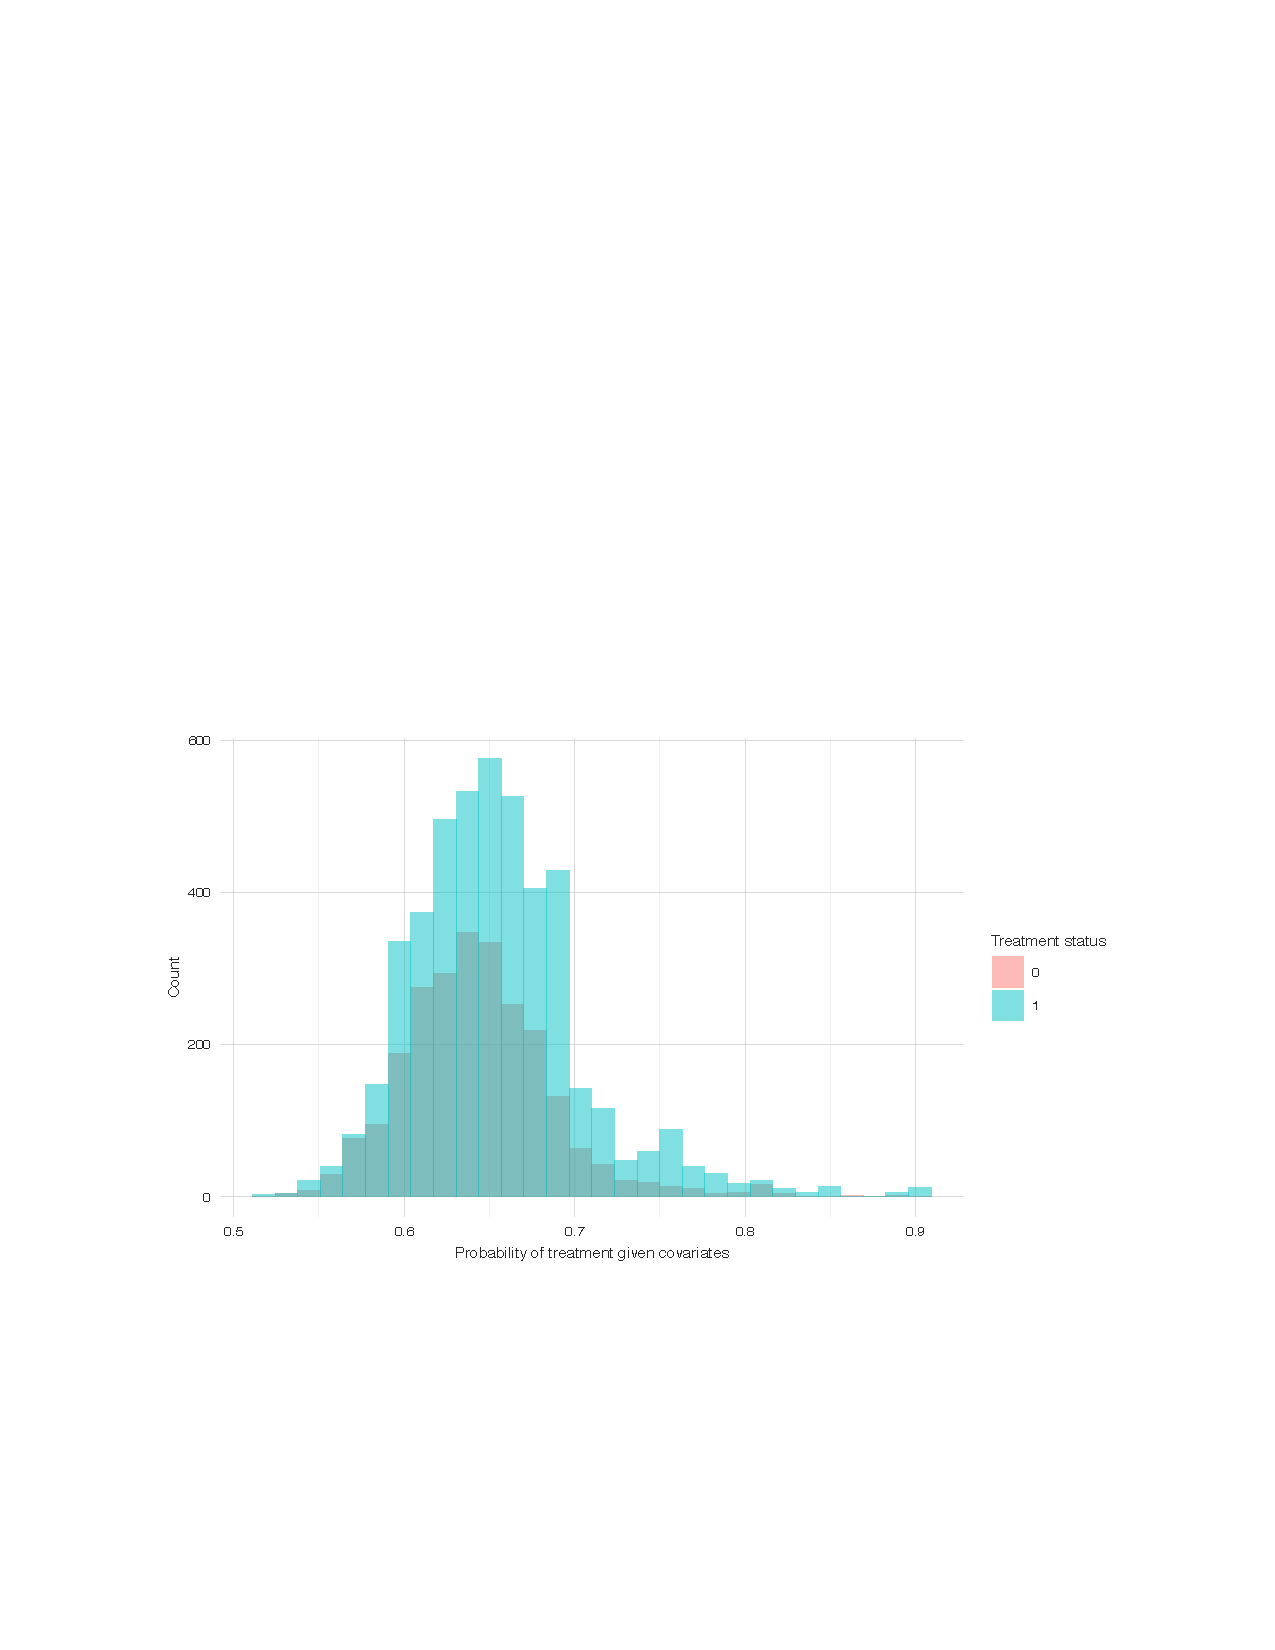
\includegraphics[height=0.5\paperheight]{figures/results_fig.pdf}
    \caption{Figure caption}
    \end{figure}
\end{frame}

%------------------------------------------------
% Figure with wrapped text
\begin{frame}{Wrapped Figure}
    \begin{wrapfigure}{r}{0.4\textwidth}
    \centering
    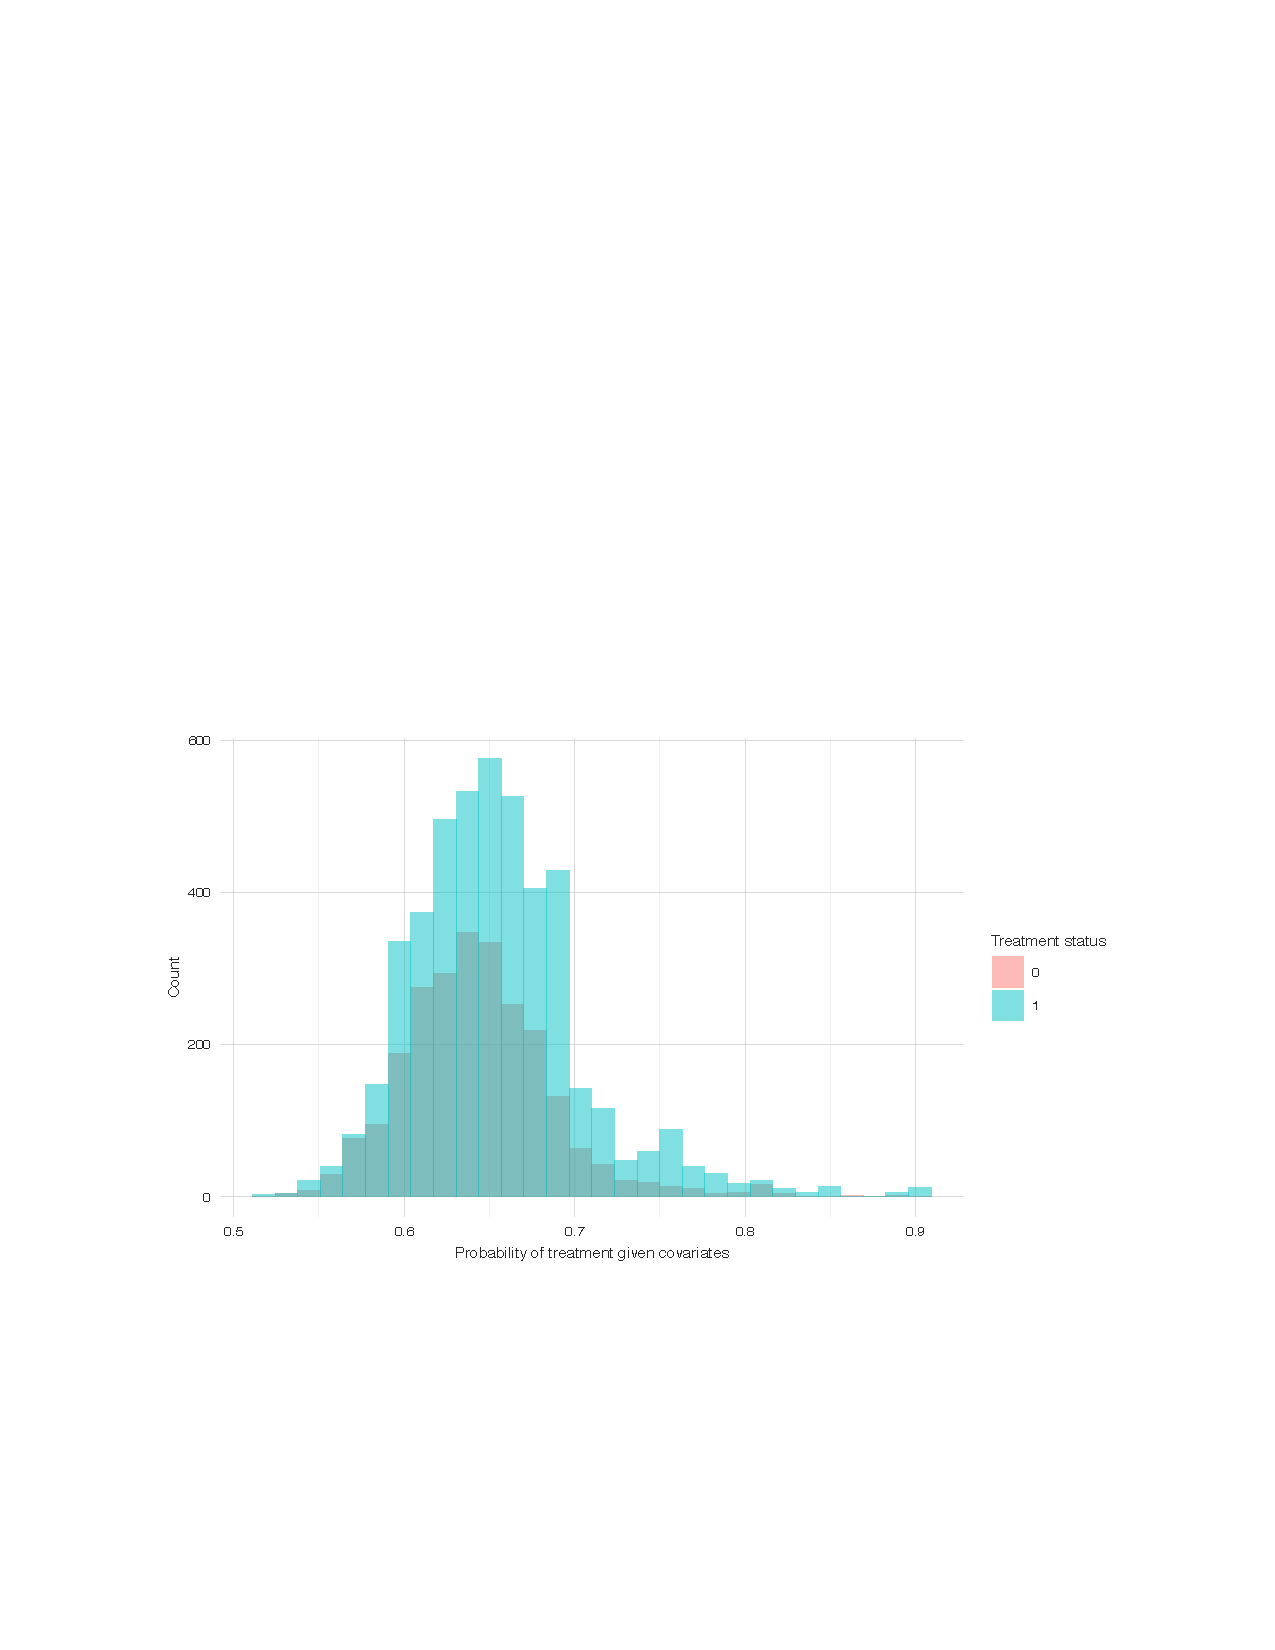
\includegraphics[width=0.4\textwidth]{figures/results_fig.pdf}
    \caption{Figure caption}
\end{wrapfigure}
"Lorem ipsum dolor sit amet, consectetur adipiscing elit, sed do eiusmod tempor incididunt ut labore et dolore magna aliqua. Ut enim ad minim veniam, quis nostrud exercitation ullamco laboris nisi ut aliquip ex ea commodo consequat. Duis aute irure dolor in reprehenderit in voluptate velit esse cillum dolore eu fugiat nulla pariatur. Excepteur sint occaecat cupidatat non proident, sunt in culpa qui officia deserunt mollit anim id est laborum.Sed ut perspiciatis unde omnis iste natus error sit voluptatem accusantium doloremque laudantium, totam rem aperiam.
\end{frame}
%------------------------------------------------
% Section divider frame
\makesection{Citations and References}

%------------------------------------------------
% Citations
\begin{frame}[fragile] % Need to use the fragile option when verbatim is used in the slide
    \frametitle{Citation}
    An example of the \verb|\cite| command to cite within the presentation:\\~

    This statement requires citation \cite{p1}.
\end{frame}

%------------------------------------------------
% Refenrenced
\begin{frame}{References}
\bibliographystyle{alpha}
\bibliography{../refs}
\end{frame}

%----------------------------------------------------------------------------------------
% Final PAGE
% Set the text that is showed on the final slide
\finalpagetext{Thank you for your attention}
%----------------------------------------------------------------------------------------
\makefinalpage
%----------------------------------------------------------------------------------------
\end{document}